\chapter{Disertantes}

Presentamos aqu� los disertantes de cada evento con una breve biograf�a y sus campos de investigaci�n.

\section*{Encuentro de Estudiantes de �ptica y Fotof�sica (EEOF)}

%%%%%%%%%%%%%%%%%%% STEFANI
\subsection*{Fernando Stefani}


\begin{tabular}{ l l}
% \newcolumntype{S}{>{\centering\arraybackslash} m{.4\linewidth} }
{\multirow{3}{*}{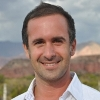
\includegraphics[width=0.08\textwidth]{fstefani}}} &  Applied nanoPhysics Group. \\
 & Physics Department of the University of Buenos Aires. \\
 & fernando.stefani@df.uba.ar
\end{tabular}

\subsubsection*{Research fields}

\begin{itemize}
\item    Metallic, semiconducting and magnetic nanoparticles
\item    Organic fluorophores
\item    Conjugated polymers
\item    Supramolecular structures
\item    Hybrid nanobiosystems
\item    Proteins and DNA

\end{itemize}

\subsubsection*{Short biography}
\begin{itemize}    
\item   born 19.11.1975 in Buenos Aires
\item   Materials Engineering studies at the Instituto de Tecnolog�a Prof. Jorge Sabato (IT) - Buenos Aires, Argentina
\item   2004 PhD at the Max-Planck-Institute for Polymer Research (MPIP, Prof. Dr. W. Knoll) - Mainz, Germany
\item   2004-2006 Postdoc at the MPIP (Prof. Dr. W. Knoll) - Mainz, Germany
\item   2006-2008 Research fellow at the Institute of Photonic Sciences (ICFO, Prof. Dr. Niek van Hulst) - Barcelona, Spain
\item   2008-2009 Group leader the Physics Department of the Ludwig-Maximilians-Universit�t M�nchen (LMU, Prof. Dr. Jochen Feldmann) - Munich, Germany
\item   Since 2009 Associate Researcher of the National Research Council (CONICET) and head of the Applied nanoPhysics Group at the Physics Department of the University of  Buenos Aires (UBA) - Buenos Aires, Argentina
\item   Since 2010 Associate Professor of the Physics Department of the University of Buenos Aires (UBA), Buenos Aires, Argentina.
\item   Since 2011 leader of a Max-Planck-Society Partner Group in collaboration with the Nanobiophotonics group of Prof. Stefan W. Hell at the MPI biophysikalische Chemie (G�ttingen).
\end{itemize}


%%%%%%%%%%%%%%%%%%%%%%%%% BRAGAS
\subsection*{Andrea Bragas}

\begin{tabular}{ l l}
% \newcolumntype{S}{>{\centering\arraybackslash} m{.4\linewidth} }
{\multirow{3}{*}{
\includegraphics[width=0.08\textwidth]{abragas}}} & Quantum Electronics Laboratory.  \\
 & Physics Department, FCEyN, UBA. Argentina. \\
 & bragas@df.uba.ar
\end{tabular}


\subsubsection*{Research fields}

\begin{itemize}
\item   High resolution optical microscopy
\item   Plasmonic probes
\item   Vibrations of plasmonic objects and ensembles
\item   Linear and nonlinear optical properties of nanomaterials.
\end{itemize}

\subsubsection*{Short biography}
    
Andrea Bragas is one of the heads of the Quantum Electronics Lab at the University of Buenos Aires and professor at the School of Sciences. Her current research fields are focused on the fabrication, study and control of different isolated and interacting plasmonic objects with the aim of their application to high-resolution microscopies, chemical and biological sensing, bio-imaging, and development of nano-light sources. \\


%%%%%%%%%%%%%%%%%%%%%%%%%%%% MAIER
\subsection*{Stefan Maier}

\begin{tabular}{ l l}
% \newcolumntype{S}{>{\centering\arraybackslash} m{.4\linewidth} }
{\multirow{3}{*}{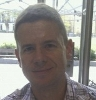
\includegraphics[width=0.08\textwidth]{smaier}}} & Nanoplasmonics group.  \\
 & Imperial College, London, UK. \\
 & s.maier@imperial.ac.uk
\end{tabular}


\subsubsection*{Research fields}

\begin{itemize}
\item    Nanocavities: Fundamentals and applications in energy concentration and biosensing 
\item    Optical and THz Metamaterials 
\item    Nanoantennas and enhanced Light/Matter coupling 
\item    Active Plasmonics and Plasmon Waveguides
\end{itemize}

\subsubsection*{Short biography}
    
Stefan Maier is Professor of Nanophotonics in the Department of Physics at Imperial College London, and co-director of the College's Centre for Plasmonics and Metamaterials. He obtained his PhD in Applied Physics at 2003 at the California Institute of Technology. Stefan has published over 130 papers in plasmonics and nanophotonics, is a fellow of OSA, and was awarded the Sackler Prize in the Physical Sciences and the Paterson Medal of the Institute of Physics. He further holds a Royal Society Wolfson Research Merit Award.\\


%%%%%%%%%%%%%%%%%%%%%%%%%% MENON
\subsection*{Rajesh Menon}

\begin{tabular}{ l l}
% \newcolumntype{S}{>{\centering\arraybackslash} m{.4\linewidth} }
{\multirow{3}{*}{
\includegraphics[width=0.08\textwidth]{rmenon}}} & Laboratory for Optical Nanotechnologies.  \\
 & University of Utah, Utah, USA. \\
 & rmenon@eng.utah.edu
\end{tabular}

\subsubsection{Research fields}
\begin{itemize}
\item Absorbance Modulation Optical Lithography (AMOL) 
\item Patterning via Optical Saturable Transformations (POST) 
\item Ultra-high efficiency photovoltaics via Diffractive Spectrum Separation 
\item Optimized Nanophotonics for efficient ultra-thin-film photovoltaics 
\item 3D tracking of surgical instruments 
\end{itemize}

\subsubsection{Short biography}

Rajesh Menon has pioneered several technologies that will enable far-field optics to manipulate and image matter with nanoscale resolution, something that was thought impossible until a few years ago. His research has spawned over 50 publications, over 30 patents, and 2 spin-off companies. He has led several projects in nanopatterning and nanoscopy with support from DARPA, the NSF, US Air Force, and the MIT Deshpande Center for Technological Innovation. Among his honors are an NSF CAREER Award (2011) and the International Commission for Optics Prize (2009).\\
He currently directs the Laboratory for Optical Nanotechnologies at the University of Utah. Prior to that, Prof. Menon was a research engineer at MIT's Research Laboratory of Electronics, where he remains a research affiliate. He holds S.M. and Ph.D. degrees from the Department of Electrical Engineering and Computer Science at MIT. In addition, he served as the Chief Technology Officer of LumArray, a company he co-founded with colleagues at MIT. \\

\subsubsection{Presentation: Circumventing the far-field diffraction limit in optical nanopatterning and imaging}

A technique for creating deterministic structural complexity is essential to achieve high functionality at the
nanoscale, whether in electronics, photonics, or molecular biology. Scanning-electron-beam lithography (SEBL) is
the most widely used method in research, but it has a number of drawbacks. SEBL tends to be slow, expensive,
prone to placement errors, and not compatible with organics and biological material. Ideally one would prefer to
employ benign photons in the visible or near IR range for such patterning. However, the so-called far-field
diffraction barrier (first realized by Abb�) limits the smallest feature achievable by wavelength, $\lambda$ to $\sim \lambda / 4$. The
spacing between nearest-neighbor patterns cannot be smaller than $\sim \lambda / 4$.
In this presentation, I will review the approaches for nanoscale imaging in fluorescence microscopy.
Furthermore, I will describe two distinct approaches being investigated in my laboratory to circumvent the far-field
diffraction limit and thereby enable optical nanopatterning with feature spacings smaller than $\lambda / 4$.

\vspace{0.5cm}

\textbf{References}

[1] T. L. Andrew, H. Y. Tsai, and R. Menon, ``Confining light to deep subwavelength dimensions to enable optical nanopatterning'', Science 324(5929), 917-921 (2009).

[2] R. Menon and H. I. Smith, ``Absorbance-modulation optical lithography'', J. Opt. Soc. Am. A 23(9), 2290-2294 (2006).

[3] F. Masid, T. L. Andrew and R. Menon, ``Optical patterning of features with spacing below the far-field diffraction limit using absorbance modulation'', Opt. Exp. 21, 4 5209-5214 (2013). 

[4] H-Y. Tsai, S. W. Thomas, III and R. Menon, ``Scanning optical nanoscopy with optically confined probe'', Opt. Exp. 18(15), 16015 (2010).

[5] N. Brimhall, T. L. Andrew, R. V. Manthena and R. Menon, ``Breaking the far-field diffraction limit in optical nanopatterning via repeated photochemical and electrochemical transitions in photochromic molecules'', Phys. Rev. Lett. 107, 205501 (2011).

[6] P. Cantu, N. Brimhall, T. L. Andrew, R. Castagna, C. Bertarelli and R. Menon, ``Subwavelength nanopatterning of photochromic diarylethene
films'', Appl. Phys. Lett. 100, 183103 (2012).\\

